\chapter{Implementazione}

	Le due applicazioni sviluppate mirano a soddisfare le stesse richieste e presentano perciò una similarità molto stretta a livello di tecnologie utilizzate.
	Nel corso di questo capitolo verrà presentata dapprima l'applicazione monolitica, analizzandone i servizi offerti, la struttura interna e le scelte progettuali compiute;
	in seguito si passerà all'analisi del sistema a microservizi, concentrandosi sul processo di decomposizione del problema generale.
	
	L'applicazione espone complessivamente 5 servizi
	
	\begin{enumerate}
		\item \emph{Autenticazione}:
			Autentica gli utenti e verifica la validità dei token presentati.
		
		\item \emph{Gestione clienti}:
			Permette la registrazione di nuovi clienti.
			
		\item \emph{Gestione ordini}:
			Permette la generazione di nuovi ordini.
			
		\item \emph{Gestione pagamenti}:
			Gestisce il pagamento degli ordini.
			
		\item \emph{Spedizioni}:
			Permette di generare nuove spedizioni e verificare lo stato di una spedizione esistente.
	\end{enumerate}
	

\section{Autenticazione e autorizzazione}

	Gli utenti devono poter compiere solo le operazioni per le quali sono autorizzati sulla base del proprio tipo di utente, un cliente non deve per esempio poter rifornire il magazzino.
	Per questo motivo ad ogni richiesta inviata tramite API viene aggiunto un token JWT con quattro \emph{claim} privati: \texttt{badge\_n}, il numero di tessera del cliente, \texttt{created}, data e ora di creazione, \texttt{expires}, data e ora di scadenza, \texttt{role}, tipologia di utente.
	
	Il token è rilasciato durante la fase di login ed ha una validità di trenta minuti, superata la quale occorre autenticarsi nuovamente.
	Il processo di login segue i seguenti passi:
	
	\begin{enumerate}
		\item L'applicazione riceve una richiesta POST sul percorso \texttt{/login} in cui sono forniti email e hash della password (generato secondo l'algoritmo SHA-3) dell'utente che richiede di autenticarsi.
		
		\item Viene interrogato il database e vengono recuperate le informazioni associate all'utente sulla base dell'email fornita.
		
		\item Se lo hash presente nel database e quello fornito coincidono, viene generato il token inserendo tutti i claim sopra elencati.
		
		\item Il token viene firmato e restituito al client.
	\end{enumerate}
	
	Il token è firmato utilizzando l'algoritmo a chiave segreta HS256, procedura fondamentale al fine di garantire l'autenticità del token stesso quando questo sarà ripresentato.
	
	
\section{Database}

	Il database si compone di sei tabelle (vedi Figura \ref{fig:dbSchema}):
	
	\begin{itemize}
		\item \emph{Articles}: modella il magazzino, contiene i prodotti e le relative quantità.
			\begin{itemize}
				\item \emph{barcode}: codice a barre univoco dell'articolo;
				\item \emph{name}: nome dell'articolo;
				\item \emph{quantity}: quantità presente in magazzino;
				\item \emph{unit\_price}: costo unitario del prodotto.
			\end{itemize}
			Per la colonna \emph{quantity} si è definito il vincolo \texttt{positive\_quantity\_remaining\_check}, il quale impedisce che la quantità residua di un prodotto assuma valori negativi.
			\label{sec:quantityCheck}
		
		\item \emph{Customers}: elenco dei clienti registrati.
			\begin{itemize}
				\item \emph{customerid}: id univoco dell'utente;
				\item \emph{surname}: cognome;
				\item \emph{badge\_n}: numero di tessera;
				\item \emph{sex}: sesso;
				\item \emph{dob}: data di nascita;
				\item \emph{email}: email;
				\item \emph{password\_hash}: codice hash della password;
				\item \emph{customerrole}: tipologia di utente (vedi tabella successiva).
			\end{itemize}
			
		\item \emph{OrderItems}: contiene gli articoli acquistati in ogni ordine.
			\begin{itemize}
				\item \emph{articleid}: codice a barre dell'articolo acquistato;
				\item \emph{orderid}: id dell'ordine in cui è stato acquistato l'articolo;
				\item \emph{quantity}: quantità acquistata.
			\end{itemize}
			
		\item \emph{Orders}: contiene gli ordini effettuati.
			\begin{itemize}
				\item \emph{orderid}: id univoco dell'ordine;
				\item \emph{badge\_n}: numero di tessera del cliente che ha effettuato l'ordine;
				\item \emph{orderdate}: data ed ora in cui è stato generato l'ordine;
				\item \emph{total\_price}: prezzo complessivo dell'ordine;
				\item \emph{orderstate}: stato dell'ordine (vedi tabella successiva).
			\end{itemize}
			
		\item \emph{orderstate}: contiene gli stati definiti per un ordine.
			Essi sono rappresentati in una tabella a parte al fine di garantire coerenza nel database e facilità di comprensione e manutenzione.
			\begin{itemize}
				\item \emph{id}: numero intero associato allo stato;
				\item \emph{statename}: nome dello stato;
			\end{itemize}
			
		\item \emph{Roles}: contiene i ruoli definiti per gli utenti.
			Valgono le stesse considerazioni fatte per la tabella precedente.
			\begin{itemize}
				\item \emph{rolename}: nome del ruolo
			\end{itemize}
		
	\end{itemize}
	
	\begin{figure}[tbp]
		\centering
		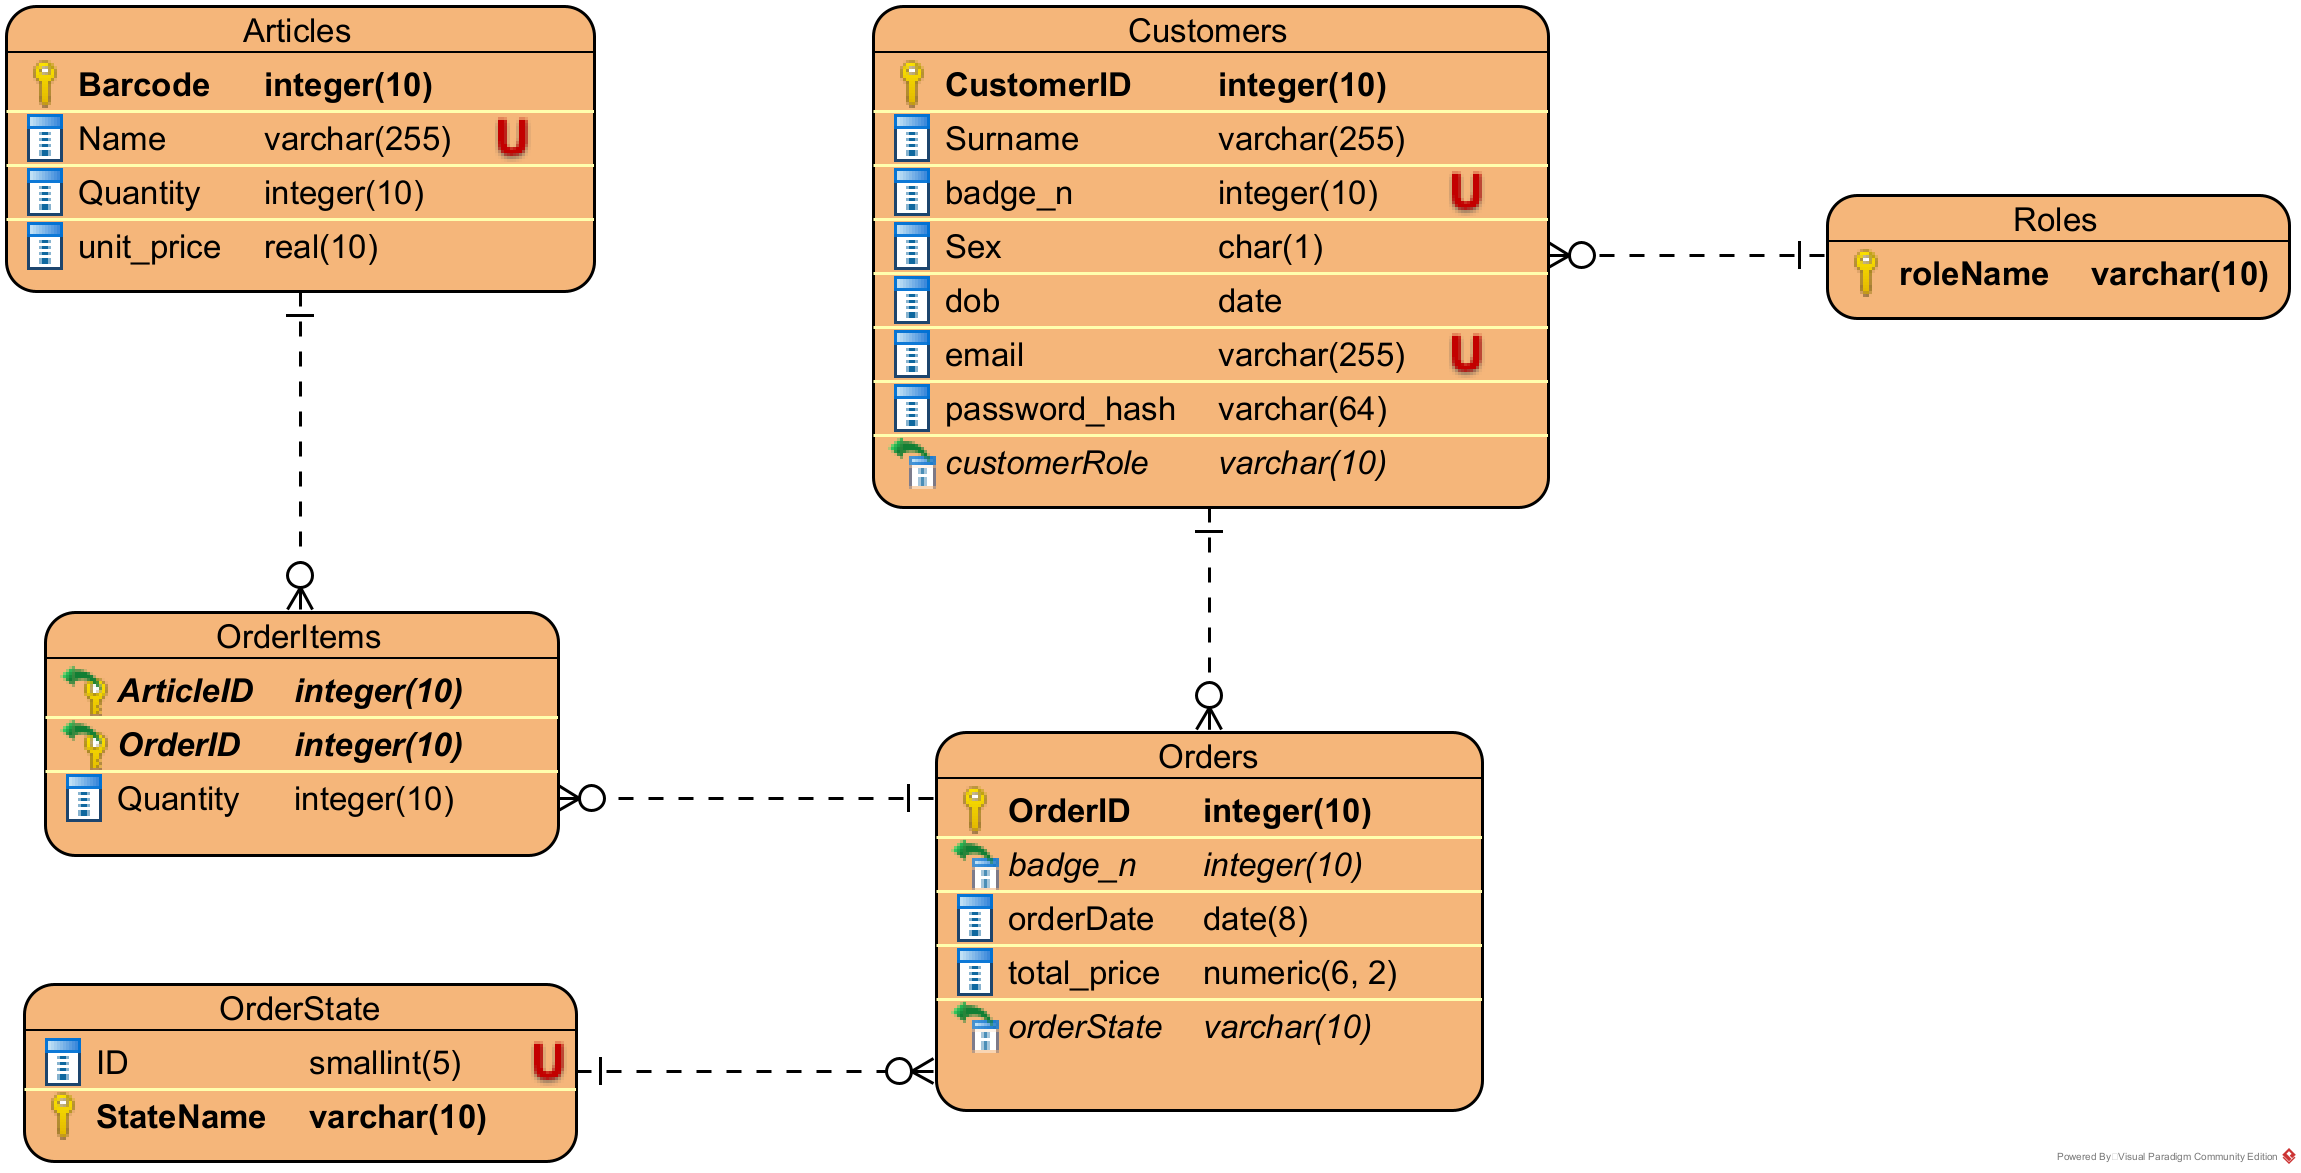
\includegraphics[width=\textwidth]{img/cap4/ER-Diagram.png}
		\caption{Schema del database}
		\label{fig:dbSchema}
	\end{figure}
	
	
\section{Esecuzione delle richieste}

	Le richieste ricevute sono eseguite nel seguente modo:
	
	\begin{enumerate}
		\item Vengono verificati la validità del token fornito e i permessi dell'utente ad effettuare la richiesta, se uno di questi due controlli fallisce viene inviata direttamente una risposta di errore.
		
		\item La gestione della richiesta viene demandata alla classe specifica, che interroga il database se necessario e predispone un oggetto JSON di risposta.
		Ogni classe dispone dei permessi in scrittura sul database, si è compiuta questa scelta al fine di evitare i colli di bottiglia tipici di una gestione centralizzata.
		
		\item Viene generata la risposta, restituendo la risorsa richiesta in formato JSON insieme a un codice di stato (\emph{status code}).
		Il codice di stato è utile per identificare l'esito positivo o negativo della richiesta, inserendo eventualmente l'errore all'interno di una macro categoria.
	\end{enumerate}
	
	

\section{Evoluzione dello stato di un ordine}
	
	Sono definiti sei stati in cui può trovarsi un ordine, si riporta il diagramma a stati finiti in Figura \ref{fig:diagStatoOrdine}.
	
	\begin{itemize}
		\item \emph{Created}: L'ordine è stato ricevuto.
		\item \emph{Confirmed}: L'ordine può essere soddisfatto, i prodotti acquistati sono stati registrati.
		\item \emph{Cancelled}: Non è possibile soddisfare l'ordine, almeno un prodotto è presente a magazzino in quantità insufficiente.
		\item \emph{Paid}: \`E stato ricevuto il pagamento.
		\item \emph{Refused}: Il pagamento è stato rifiutato.
		\item \emph{OnDelivery}: L'ordine è stato spedito.
	\end{itemize}
	
	\begin{figure}[tbp]
		\centering
		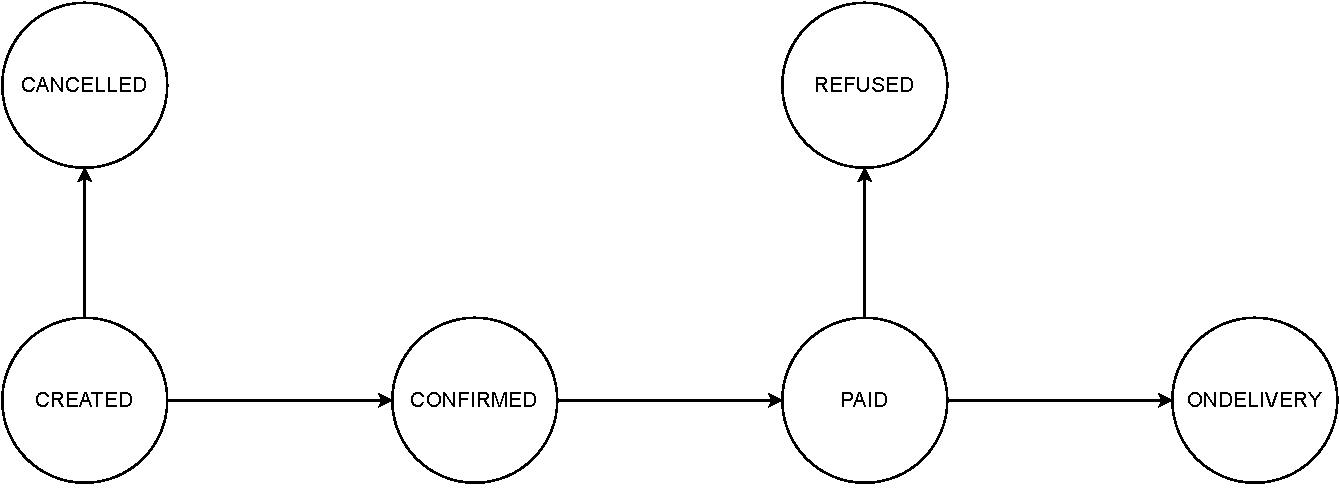
\includegraphics[width=0.9\textwidth]{img/cap4/statiOrdine.pdf}
		\caption{Diagramma a stati finiti degli stati definiti per un ordine}
		\label{fig:diagStatoOrdine}
	\end{figure}
	
	Il processo di creazione di un nuovo ordine ha inizio con l'arrivo di una richiesta POST all'API sul percorso \texttt{/newOrder} e può essere effettuato solamente da utenti di tipo \emph{customer}.
	Il corpo della richiesta deve essere in formato JSON e contenere un array di prodotti selezionati e la relativa quantità;
	la struttura deve essere quella riportata nel Codice \ref{lst:json_newOrder}.
	
	\begin{listing}[tb]
		\inputminted{json}{codici/cap4/nuovoOrdine.json}
		\caption{Struttura del corpo della richiesta per la creazione di un nuovo ordine}
		\label{lst:json_newOrder}
	\end{listing}
	
	Non è necessario specificare l'identificativo dell'utente, in quanto questa informazione, insieme al tipo di utente, è già presente all'interno del token ed è recuperata automaticamente.
	I passaggi successivi riguardano:
	
	\begin{enumerate}
		\item Viene registrato il nuovo ordine nella tabella \emph{Orders} del database, il quale si occupa di assegnare un id univoco.
		Lo stato dell'ordine è impostato su \emph{created} finché non ha l'id assegnato e viene in seguito modificato in \emph{created}.
		
		\item Vengono prelevati i prodotti ordinati dal magazzino, modificando le quantità residue nella tabella \emph{Articles}.
		Se si tenta di rimuovere un numero di prodotti superiore a quelli residui presenti in magazzino viene generata un'eccezione per la violazione del \emph{vincolo check} spiegato alla Sezione \ref{sec:quantityCheck};
		il database esegue il rollback e lo stato dell'ordine è impostato su \emph{Cancelled}.
		
		\item Vengono registrati tutti i prodotti ordinati con la quantità associata nella tabella \emph{OrderItems} del database.
		
		\item Viene calcolato il prezzo finale dell'ordine e memorizzato nella tabella \emph{Orders}.
	\end{enumerate}
	
	Se tutto va a buon fine all'utente viene comunicata la somma da pagare e lo stato dell'ordine è modificato in \emph{Confirmed}.
	

	
\section{Implementazione dei microservizi}

	L'applicazione a microservizi nasce dal codice dell'applicazione monolitica, ma lo riorganizza in unità indipendenti sulla base dei diversi servizi offerti.
	Al fine di evitare colli di bottiglia dovuti alla presenza di un singolo punto d'ingresso per le richieste, ogni microservizio espone delle proprie API.
	
	\begin{figure}[tbp]
		\centering
		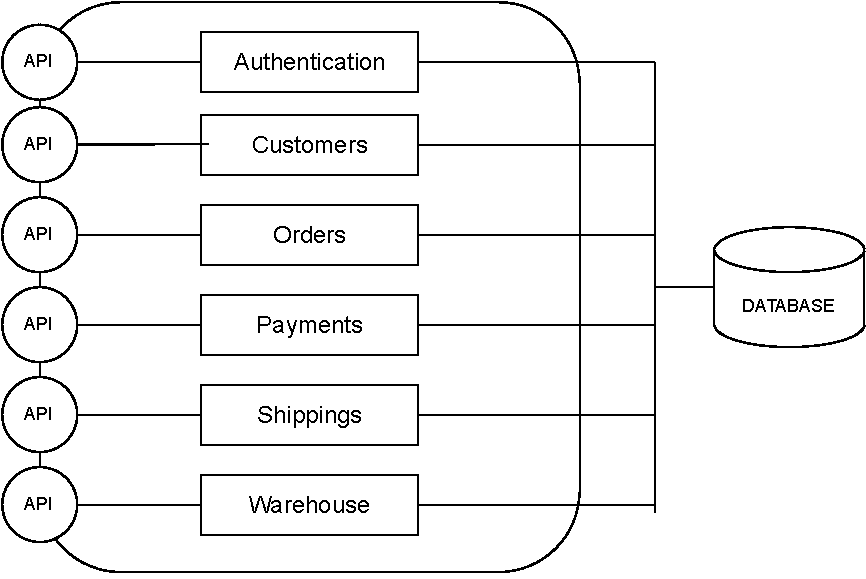
\includegraphics[height=0.5\textwidth]{img/cap4/microservizi.pdf}
		\caption{Struttura del sistema a microservizi}
		\label{fig:microservizi}
	\end{figure}
	
	Sono stati sviluppati sei microservizi, uno schema generale del sistema è mostrato in Figura \ref{fig:microservizi}:
	
	\begin{itemize}
		\item \emph{Authentication}:
			Gestisce l'autenticazione dell'utente e controlla la validità dei token.
			Espone API con metodo POST sul percorso \texttt{/login} alla porta 5000.
		
		\item \emph{Customers}:
			Permette l'iscrizione di nuovi utenti, tramite una API con metodo POST alla porta 5005 sul percorso \texttt{/registerCustomer}.
		
		\item \emph{Orders}:
			Gestisce il processo di creazione di un nuovo ordine.
			Espone API con metodo POST alla porta 5002 sul percorso \texttt{/newOrder}.
		
		\item \emph{Payments}:
			Gestisce la procedura di pagamento.
			Espone API con metodo POST alla porta 5003 sul percorso \texttt{/payOrder}	
		
		\item \emph{Shippings}:
			Genera nuove spedizioni e permette di controllare lo stato di una spedizione.
			Espone API con metodo POST alla porta 5004 sul percorso \texttt{/trackOrder}
		
		\item \emph{Warehouse}:
			Gestisce il magazzino.
			Ha una propria API attiva sulla porta 5001 al percorso \texttt{productsList}, con metodo GET per richiedere la lista dei prodotti presenti in magazzino, POST per caricare nuovi prodotti.
		
	\end{itemize}

























	
	